\section{Overview pyramid}

\subsection{On what metrics does the system scores well or bad. How does it impact quality attributes ? What is the impact of the systems score on these metrics on quality attributes
such as maintainability, extensibility... ?}

\begin{itemize}
    \item The ANDC metric is too high. It denotes high subclass coupling which makes adding features in subclasses more diffcult. It is also more difficult to maintain a large hierarchy of classes
    \item The AHH metric is too high. It takes more time to compute due to dynamic binding of overrided methods
    \item The NOM/NOC metric is low because the project is small. There are not many methods. The project is thus easily extensible but care should be taken that this metric stay low
    \item The LOC/NOM metric is high thus the methods should be split into more modular methods to improve maintenance. This can be done without impact on the quality of the code because the previous metric (NOM/NOC) is low
    \item The CYCLO/LOC metric is low because the code is very flat. It is good because there are less edge cases to test. The code is easy to understand and maintain. The project mainly consists in adding and storing data in a database.
    \item The CALL/NOM metric is high but the FANOUT/CALL metric is low. It denotes that operations mostly use operations from the same class. The coupling is thus low and it helps maintenance and extensibility.
    \item The FANOUT/CALL is low because thanks to facades the code is well decoupled.
\end{itemize}

The project scores particularly well on the CYCLO, NOM and FANOUT metrics. Overall it means that the code is flat with a low number of methods that call mainly methods from the same class.

\subsection{How is each metric computed ?}

\begin{itemize}
    \item ANDC : computes the sum of the number of derived class for each superclass and divide by the number of classes
    \item AHH : computes for each class with no parent (called root class) the number of classes to the lowest subclass and divide by the number of root classes
    \item NOM : compute the sum of the number of methods of each class
    \item NOC : the number of classes
    \item LOC : the number of lines of code without comments lines
    \item CYCLO : create a tree of all the condition branchments in the code and compute the number of leaves of the tree
    \item FANOUT : compute the sum of distinct classes used in each operation
    \item CALL : compute number of distinct other operations called in each operation
\end{itemize}

\subsection{Important points on the overview pyramid diagram}

\begin{figure}[H]
    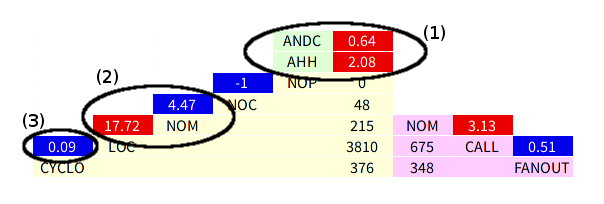
\includegraphics[width=\textwidth]{OverviewPyramid_annotated.png}
    \caption{\label{fig:pyramid}Overview pyramid with emphasis on important points}
\end{figure}

\begin{enumerate}
    \item The hierarchy is too big in both width and height. It denotes a strong subclass coupling. The same features could probably be reached without inheritance.
    \item The number of lines of code per method is too high. Because the number of methods is not high, each method could be split into smaller methods to increase modularity and facilitate maintenance and extensibility.
    \item There are not many conditional branchements, which is very good for both unit tests and integration tests. It also facilitates the reading and understanding of the code.
\end{enumerate}

\section{System attraction}
On the figure below, classes are represented as big black dots, methods as red dots and attributes as blue dots. The lines show the use of class methods and attributes by other classes and methods. In order to obtain this diagram in Moose, we choose the category \textbf{All model classes}, then select \texttt{Visulaize > System attraction}

\begin{figure}[H]
    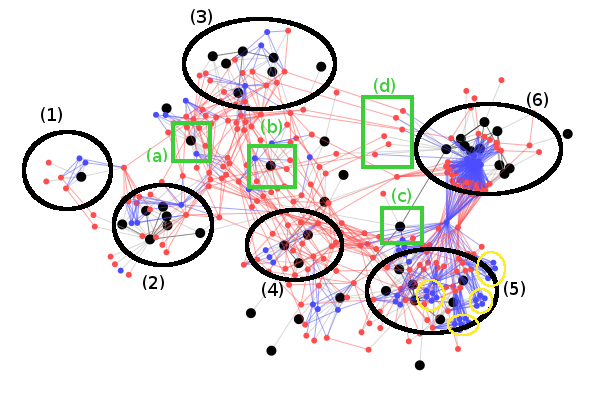
\includegraphics[width=\textwidth]{Attraction_annotated.png}
    \caption{\label{fig:attraction} Attraction diagram}
\end{figure}

\paragraph*{}
\begin{minipage}{0.6\textwidth}
  \begin{enumerate}
    \item InternetFrontend
    \item Pages (\begin{scriptsize}\texttt{LoginPage, QueryPage, ...}\end{scriptsize})
    \item Managers (\begin{scriptsize}\texttt{UserManager, ApplicationManager, ...}\end{scriptsize})
    \item Databases (\begin{scriptsize}\texttt{RawDatabase, RegularDatabase}\end{scriptsize})
    \item Database entries (\begin{scriptsize}\texttt{Book, Article, ...}\end{scriptsize})
    \item Registrations (\begin{scriptsize}\texttt{Administrator, CheapSubscription, ...}\end{scriptsize})
  \end{enumerate}
\end{minipage}\hfill
\begin{minipage}{0.3\textwidth}
  \begin{enumerate}[label=\alph*]
    \item ApplicationFacade
    \item DatabaseFacade
    \item Data
    \item UserProfile accessors
  \end{enumerate}
\end{minipage}

\paragraph*{}\textit{The other classes are not relevant for a complex system analysis (unit tests for instance).}

At first sight, this diagram looks like a spider web, with a few recognizable clusters of classes. The overall project does not seem to be well organized, because classes of different concerns seem to be linked together. The 3-tier architecture is not well implemented, otherwise we would clearly see the 3 layers on the visualization. Let's take a closer look.

\subsection{Users}
The cluster \texttt{(6)} contains the User classes, which are tightly grouped together. This indicates that they are highly coupled, because of their common ancestor: \texttt{Registration}. Interestingly enough, all of these classes are only used through a few attributes accessors (cluster \texttt{(d)} and right of cluster \texttt{(c)}), which means that they are loosely coupled to the rest of the system.

\subsection{Facades}
The \texttt{ApplicationFacade} (cluster \texttt{(a)}) and the \texttt{DatabaseFacade} (cluster \texttt{(b)}) do not fulfill their roles. A lot of links bypass them, which indicates that users of the facades are aware of what should be hidden behind the facade. In the ideal case, we should only see those classes as articulation nodes between clusters on the diagram.

\subsection{Data}
The data classes (cluster \texttt{(5)}) are also clearly identifiable. They are mostly accessed through the databases (cluster \texttt{(4)}). We attribute the \textit{spider web} feeling around the cluster to the tests cases (below cluster \texttt{(4)}). These data classes are essentially models (high number of attributes, few methods) as it can be seen in the small yellow clusters.

\section{Custom system complexity}
